% Stage Report II (English). Build with TeXLive (two passes), in docs/report/stage_report_2/:
%   pdflatex stage_report_2.tex && pdflatex stage_report_2.tex
% Every number re-derived from artifacts 2026-10-01; see runs/analysis/report2_numbers.txt.
\documentclass[11pt]{article}
\usepackage[margin=1in]{geometry}
\usepackage{amsmath,amssymb}
\usepackage{booktabs}
\usepackage{multirow}
\usepackage{graphicx}
\usepackage{xcolor}
\usepackage[hidelinks]{hyperref}
\emergencystretch=3em

\title{\bfseries Two Attacks on the Dead-Nucleus Detection Deficit:\\
Detection-First Architectures Do Not Transfer, and $2\times$\\
Resolution Buys Dead at a Priced Trade\\[6pt]
\large Stage Report II (Course Project bdd26)}
\author{}
\date{October 1, 2026}

\begin{document}
\maketitle
\section*{Audit and follow-up v2: October 2, 2026}
\textbf{This addendum supersedes conflicting historical claims and the first audit's v1 results.}
The initial M/S repair fixed class indexing and background perimeter contamination, but
pre-merge review found that shared contacts were overwritten between directions and that
validation reconstructed lossy GT class channels. Both are now fixed. P0--P2 and their
bootstrap were rerun on CPU with the same validation-only menus and cached predictions;
old outputs remain archived, not relabelled as corrected experiments.

The nine historical x2 runs were \emph{not} a complete three-distinct-seed grid:
split 2 used $\{19,1,1\}$; baseline coverage was 3/1/1. Run spread is not fully paired
seed uncertainty. mPQ$^+$ is class-aware, $F_c$ mixes detection and typing errors, and
\texttt{missed\_bg} means maximum IoU below 0.1, not necessarily zero overlap. Released
validation-selected checkpoints differ from our own final-checkpoint protocol;
a uniform paper gap alone does not prove pipeline correctness.

\begin{center}\small
\begin{tabular}{lrrrr}
\toprule
Corrected v2, seed 19, three splits & mPQ & bPQ & Dead PQ & strict Dead PQ\\
\midrule
x1 + M/S & .4998 & .6656 & .1767 & .1340\\
x2 + scaled decode + M/S & .4906 & .6601 & .1850 & .1249\\
Conservative additions (P2) & .4999 & .6652 & .1835 & .1371\\
\bottomrule
\end{tabular}
\end{center}

P2 freezes rules on validation and retains identity on split 1. Against x1+M/S v2,
mean changes are $+$.000072 mPQ, $-$.000448 bPQ, $+$.006846 Dead PQ and
$+$.003003 strict Dead PQ. Only split 3's Dead gain excludes zero in the paired
image bootstrap; training-seed robustness is untested, and strict Dead has no CI here.
Strict mPQ decreases slightly. This is a candidate, not an established overall win;
using both models' predictions has an unmeasured deployment cost.

P1 finds a transferable typing component with fixed x2 geometry (mPQ .4906 to .4974).
P3 reuses the same 128 split-1 validation images; scale mismatch degrades performance,
but this is not a full test benchmark. No new training or GPU inference was needed for v2.
See \texttt{P0\_P3\_RESULTS\_2026-10-02.md} in docs for protocols, uncertainty and provenance.
\clearpage


\begin{abstract}
Stage report I located the PanNuke \emph{Dead} (apoptotic) class deficit in
\emph{detection}---38.5\% of Dead ground-truth nuclei receive no overlapping prediction---and
showed it survives every loss-level and data-level intervention we tried, across three
dense-decoder architectures. Two escapes were left untested: the \emph{detection-first}
architecture family, whose published Dead numbers are the strongest in the literature, and
\emph{working resolution}. This report tests both under the same strict protocol (official
3-fold split, last checkpoint, validation-only tuning, artifact-aware Dead reporting).
\textbf{Line A (negative).} The released per-fold KongNet checkpoints---a six-head
CenterNet-style detector whose fold mapping we first resolve empirically---score 0.346 mPQ
under a validation-tuned decode, 11 points below the \emph{weakest} dense decoder; its
contour-cut channel is net-harmful at 40$\times$ (every optimum disables it), same-class
touching nuclei fuse (merged rate 0.12--0.18 vs 0.04--0.05 for watershed decoders),
interior-Dead miss is \emph{worse} (0.50 vs 0.35), and the paper's Dead $F_c$ 0.59 falls to
0.34. LKCell-L, the strongest released per-fold weights we could find, reproduces
$\sim$0.015 uniformly below its published numbers and, under matched conditions, is a
\emph{better segmenter but worse typer} than our CellViT-UNI baseline (bPQ $+$0.008, Dead PQ
$-$0.022): architecture strength does not convert into Dead or typing gains. \textbf{Line B
(a priced trade).} Doubling working resolution to 512\,px as a single-variable change makes
every pre-registered Dead endpoint positive (interior-Dead miss $0.35\!\to\!0.25$) but pays a
uniform bPQ tax of $-$0.026. Error analysis refutes the downsample hypothesis (that mapping
512 predictions back to 256 destroys boundaries) and traces most of the tax to a hidden
confound: the watershed decode applies \emph{fixed pixel-unit constants} (minimum object
size, Sobel aperture) that silently relax in native units at $2\times$. The pre-registered
fix---scaling those constants by the resolution factor---recovers 50--87\% of the
mPQ/bPQ/mPQ$^+$ cost while keeping---and slightly enlarging---the Dead gain; a
validation-only post-processing lever (same-class instance merging $+$ edge-sliver dropping)
then yields a strict improvement on the test folds in all 9 runs of a $3{\times}3$
split$\times$seed grid. The pre-registered seed-noise verdict on that grid: the
\emph{prices} are seed-robust ($4.7$--$5.3\times$ the largest seed std, same sign on every
run), the \emph{Dead gain} is fragile ($0.4$--$0.7\times$ the per-seed Dead std; one split's
seed-mean flips sign). Final standing: $-$0.008 mPQ / $-$0.005 bPQ buys $-$0.069
interior-Dead miss, $+$0.034 Dead $F_c$, and mPQ$^+$ parity---not a default win, an
explicitly priced trade. We conclude that the Dead deficit is not an artifact of one
architecture family: more pixels buy real detection gains, while separating---and
typing---what those pixels newly resolve remains unsolved, and pixel-unit decode constants
are a first-class confound that any resolution study must control for.
\end{abstract}

\section{Introduction}
\label{sec:intro}

Stage report I ended with a closed diagnosis: on PanNuke~\cite{gamper2019pannuke}, the Dead
(apoptotic-body) class fails at \emph{detection}, not classification. The foreground head is
silent on 83\% of missed Dead nuclei while the type branch already assigns them
P(Dead)$\approx$0.26; re-typing with a pathology VLM, training-free recovery, loss
re-weighting, copy-paste augmentation, and in-context synthesis were all null or harmful; and
the deficit was shared by all three dense-decoder architectures we evaluated (a ViT-L/16, a
full-resolution ResNet-50, a ConvNeXt decoder). Two hypotheses remained open, and this report
closes both under the same pre-registered, noise-calibrated protocol:

\begin{enumerate}
\item \textbf{Architecture (Line A):} the failure is a property of \emph{dense decoders}
(foreground + watershed). Detection-first designs that predict per-class centroids and
assemble masks around them report by far the strongest Dead numbers in the literature
(KongNet~\cite{lv2025kongnet}: per-nucleus Dead $F_c$ 0.59, vs 0.23--0.36 for our dense
models under strict decoding). If that advantage is real under matched evaluation, the Dead
deficit has an architectural fix. We test the released per-fold KongNet checkpoints
end-to-end---resolving their undocumented fold mapping empirically first---and re-evaluate
LKCell-L~\cite{cui2024lkcell}, the strongest released per-fold weights of the CellViT
lineage, in the same pipeline.
\item \textbf{Resolution (Line B):} the failure reflects the 256\,px working resolution:
Dead nuclei are small (median 107\,px vs 368 for other classes), 31\% of interior Dead nuclei
are missed, and even among Dead nuclei of at least 256\,px the miss rate is 17\%---so more
pixels should help detection regardless of decoder. We double the working resolution of the
unchanged CellViT-UNI recipe (single-variable change), then follow the error trail wherever
it leads: an initial uniform bPQ tax, a mechanism diagnosis that overturns the obvious
explanation, a pre-registered decode fix, a validation-only post-processing lever, and a
$3{\times}3$ split$\times$seed grid whose seed-noise verdict was written down before the last
runs landed.
\end{enumerate}

Contributions:

\begin{enumerate}
\item \textbf{A strict-protocol verdict on detection-first architectures} (Sec.~\ref{sec:lineA}):
KongNet's released per-fold weights, given their best validation-tuned decode, are 11 mPQ
points below the weakest dense decoder, fuse touching nuclei, and miss \emph{more} interior
Dead nuclei; the paper's Dead $F_c$ 0.59 does not replicate (0.34 strict). LKCell-L is a
better segmenter and worse typer under matched conditions. The generalizable lesson:
published Dead advantages so far reflect evaluation recipes and segmentation--typing
trade-offs rather than genuinely better Dead detection.
\item \textbf{A mechanism study of resolution in nuclei decoding}
(Sec.~\ref{sec:mechanism}--\ref{sec:du2}): the $2\times$ bPQ tax is size-axis-monotone,
not class-localised; boundary quality of matched nuclei is unchanged; and the dominant cause
is two pixel-unit constants hardcoded in the watershed decode (object-size floor, Sobel
aperture) that relax in native units when resolution doubles. Scaling them by the resolution
factor ($du2$) recovers 50--87\% of the aggregate cost. To our knowledge this confound is
undocumented in the nuclei-segmentation literature, and it applies to \emph{any} pipeline
built on the HoVer-Net post-processing stack.
\item \textbf{A pre-registered, fully replicated characterization of the priced trade}
(Sec.~\ref{sec:lever}--\ref{sec:final}): a validation-only lever (same-class
merge + edge-sliver drop, frozen constants) strictly improves the $du2$ arm on all 9
grid runs; the $3{\times}3$ seed grid separates robust prices from a fragile Dead gain; and
the final standing prices every Dead improvement in mPQ/bPQ units.
\item \textbf{Two further evaluation-methodology results}: the KongNet fold mapping of
released checkpoints can be recovered from memorization alone (train-fold detection F1 margin
$\geq$0.13, no test-fold information used); and LKCell-L's paper-to-strict gap is
\emph{uniform} ($\sim$0.015 on every headline metric), the signature of a protocol
translation rather than a pipeline error---the second released model, after HoVer-NeXt-T in
report I, whose published-to-strict gap exceeds the spacing between leaderboard neighbors.
\end{enumerate}

All results come from a single codebase and the same bit-exact evaluator; every table in
this report was re-derived from stored prediction artifacts on 2026-10-01
(script \texttt{scripts/report2\_numbers.py}; the extracted numbers are archived with the
run artifacts).

\section{Related Work}
\label{sec:related}

\paragraph{Dense-decoder lineage.} HoVer-Net~\cite{graham2019hovernet} established the
nuclear-probability / horizontal--vertical / type decomposition with watershed decoding that
CellViT~\cite{horta2024cellvit} inherited; HoVer-NeXt~\cite{hovenext} and
LKCell~\cite{cui2024lkcell} are recent variants. Report I showed this whole family shares the
Dead detection deficit.

\paragraph{Detection-first and point-prediction models.} Centroid/heatmap detectors for
nuclei go back to StarDist-class and CenterNet-style designs; KongNet~\cite{lv2025kongnet}
(a six-head EfficientNetV2-L model: per-class heatmap + regression + segmentation/contour
channels) reports the strongest published per-nucleus Dead $F_c$ (0.59) with released
per-fold weights, which is what made it the right Line-A test: the claim is specific,
checkable, and load-bearing for the "detection-first fixes Dead" hypothesis.
PromptNucSeg~\cite{promptnucseg} and CellVTA represent the prompt/adapter branch; their
released weights are queued for the same re-evaluation (Sec.~\ref{sec:status}).

\paragraph{Resolution in nuclei segmentation.} Higher input or working resolution is an
evergreen lever (CellViT-SAM-H at 512; LKCell's multi-scale large kernels; HoVer-NeXt's
pyramid), but published ablations compare end-to-end configurations rather than isolating
the resolution variable with the decode held to account. The closest antecedent to our
finding is the classic scale-space literature: watershed markers and morphological floors
are pixel-unit operators, so their effective scale changes with image resolution---a fact
that, to our knowledge, has not been called out as a confound in learned
nuclei-segmentation pipelines, where these constants are inherited verbatim from HoVer-Net's
released post-processing code.

\section{Experimental Setup}
\label{sec:setup}

\paragraph{Protocol (unchanged from report I).} PanNuke folds 1--3, official assignment
(train/val/test $=1/2/3$, $2/1/3$, $3/2/1$); last checkpoint for our trained runs, released
per-fold (validation-selected) checkpoints for the re-evaluated models; nothing is tuned on
test folds; official tissue-averaged mPQ/bPQ from our bit-exact evaluator; TTA (8 dihedral
views, HV remapped) reported separately. Dead endpoints are reported four ways as in
report I: official Dead PQ, Uterus-excluded Dead PQ (the official per-class PQ averages only
over images containing the class, and fold 3 contains 34 Uterus images near zero for every
model), per-nucleus Dead $F_c$ (12\,px centroid matching), and the interior (non-border)
Dead miss rate.

\paragraph{Released-weight re-evaluation rules (Line A).} (1) The fold mapping of released
checkpoints must be established without touching test folds: for KongNet we run each
checkpoint on 200-image subsamples of every \emph{train} fold and read the mapping off the
memorization diagonal (Sec.~\ref{sec:kongnet}). (2) Any decode thresholds are tuned on
validation folds only, with grids extended until the optimum is bracketed; test folds run
once with frozen constants. (3) Class-channel semantics of vendored decoders are verified on
train folds only (matched-pair confusion diagonal $\geq$0.97). LKCell-L uses its released
configuration (normalisation, 256\,px decode) unmodified through our shared pipeline.

\paragraph{$2\times$ working resolution (Line B).} The exact CellViT-UNI recipe with the
working resolution doubled to 512: bilinear image upsample after augmentation, nearest-neighbour
labels, prediction post-processed at 512 and downsampled to 256 for the standard evaluator
(instance type-probability tables computed at model resolution). One variable changes.
$du2$ denotes the decode fix of Sec.~\ref{sec:du2}; \emph{lever} the post-processing of
Sec.~\ref{sec:lever}. The seed grid is 3 splits $\times$ seeds \{19, 1, 2\}; baseline seeds
1/2 exist on split 1 (report I), so seed standard deviations are fully populated there and
reported per split.

\paragraph{Noise calibration (carried over, now twice validated).} Seed std of the identical
CellViT-UNI recipe: 0.0021 mPQ but 0.0074 Dead PQ (split 1); image-bootstrap CI half-width on
Dead 0.02--0.03. Verdict rules: Dead changes below $\sim$0.01--0.015 single-seed are noise;
every intervention verdict is a multi-run statement with paired, tissue-stratified image
bootstrap 95\% CIs; validation-fold decisions only. The Line-B seed-noise verdict was
pre-registered before the last grid runs landed (Sec.~\ref{sec:grid}).

\section{Line A: Detection-First Architectures Under the Strict Protocol}
\label{sec:lineA}

\subsection{KongNet: fold mapping, best decode, and a decisive negative}
\label{sec:kongnet}

\paragraph{Assets and fold mapping.} KongNet's released \texttt{KongNet\_PanNuke\_\{1,2,3\}.pth}
(176.9M parameters, tf\_efficientnetv2\_L encoder + six SMP decoders: one overall head + five
per-class heads, each with heatmap/segmentation/contour channels) ship with no fold
documentation. Running all three checkpoints on 200-image subsamples of every \emph{train}
fold gives a clean memorization diagonal (pooled detection F1, centroid pairing at 12\,px):
checkpoint $k$ wins train fold $k$ at 0.905/0.944/0.912 with margin $\geq$0.13 over both
held-out folds---\texttt{\_k.pth} is official split $k$, resolved without any test-fold
information. Class-channel semantics were verified on train folds (matched-pair class
agreement 0.97--0.99, with near-zero off-diagonal mass for Dead).

\paragraph{The contour cut is net-harmful at 40$\times$.} The released inference recipe
assembles instances as per-class segmentation-minus-contour masks. We swept the two decode
thresholds on validation folds (grids extended twice until each optimum was bracketed).
Every checkpoint's optimum \emph{disables} the contour cut entirely (contour threshold 1.0):
on checkpoint 1, disabling the cut moves validation mPQ $0.331\!\to\!0.345$ and bPQ
$0.457\!\to\!0.473$. The repo's contour-threshold-0.3 recipe over-splits nuclei at this
scale; with the cut off, the decode degenerates to plain per-class connected components.

\begin{table}[t]
\centering\small
\caption{Strict-protocol architecture table (3-split means, no TTA, last/released per-fold
checkpoints, validation-tuned decodes). Dead endpoints: official PQ, Uterus-excluded PQ,
per-nucleus $F_c$, DQ$^+$, and interior-Dead miss (share of non-border Dead GT with no
matched prediction; mean of per-split rates). HoVer-NeXt-T (report I: 0.458 mPQ / 0.637 bPQ
/ 0.136 Dead PQ) lacks artifact-derived Dead columns here. LKCell-L paper row as published.}
\label{tab:arch}
\begin{tabular}{lcccccccc}
\toprule
Model & mPQ & bPQ & mPQ$^+$ & \shortstack{Dead\\PQ} & \shortstack{Dead\\$-$Uterus} & \shortstack{Dead\\$F_c$} & \shortstack{Dead\\DQ$^+$} & \shortstack{int-Dead\\miss} \\
\midrule
KongNet (strict)     & .3460 & .4706 & .3472 & .053 & .070 & .344 & .232 & .520 \\
HoVer-Net (ours)     & .4564 & .6613 & .4430 & .127 & .152 & .230 & .275 & .404 \\
LKCell-L (strict)    & .4923 & .6729 & .5235 & .154 & .201 & .382 & .418 & .347 \\
\quad paper          & .508 & .685 & --- & .172 & --- & --- & --- & --- \\
CellViT-UNI (ours)   & .4995 & .6653 & .5178 & .176 & .218 & .359 & .396 & .372 \\
\midrule
x2 $+$ du2           & .4894 & .6583 & .5157 & .183 & .226 & .395 & .424 & .302 \\
x2 $+$ du2 $+$ lever & .4910 & .6608 & .5171 & .183 & .227 & .393 & .422 & .302 \\
\bottomrule
\end{tabular}
\end{table}

\paragraph{Test verdict.} Table~\ref{tab:arch}, top block: with the frozen best decode,
KongNet reaches \textbf{0.346 mPQ / 0.471 bPQ}---11 mPQ and 17--19 bPQ points below the
weakest dense decoder---and every pre-registered Dead endpoint fails: official Dead PQ 0.053
(dense
0.127--0.176), Uterus-excluded 0.070, interior-Dead miss 0.50 \emph{vs} 0.354 (CellViT-UNI)
and 0.413 (HoVer-Net) on the shared splits-1+3 frame. Only per-nucleus Dead $F_c$ is
mid-pack (0.344). The error profile explains why: \emph{same-class touching nuclei fuse}.
The merged-GT rate is 0.121--0.175 across splits (CellViT-UNI 0.044--0.045, HoVer-Net
0.048--0.050); with the contour cut disabled the decode cannot separate touching instances at
all, and re-enabling it costs more than it saves. This is precisely the failure geometry of
karyorrhectic Dead clusters (report I: 73--82\% of merged Dead touch another Dead): the Dead
deficit is an \emph{instance-separation} problem, not a detection-density problem, so a
detector that finds Dead nuclei but cannot cut fragment clusters converts nothing into Dead
PQ. KongNet's paper Dead $F_c$ 0.59 (their decode, their evaluation) does not survive
validation-tuned decoding; Line A is closed as a negative result.

\subsection{LKCell-L: a uniform paper gap, and segmentation--typing non-conversion}
\label{sec:lkcell}

LKCell-L (UniRepLKNet-S encoder, RepLK decoder, CellViT np/hv/tp heads) is the strongest
model with released per-fold weights in the CellViT lineage (paper: 0.508 mPQ / 0.685 bPQ /
0.172 Dead PQ). We ran its released per-fold \texttt{model\_best} checkpoints through the
shared pipeline (its normalisation, its 256\,px decode, no TTA):

\begin{itemize}
\item \textbf{The paper gap is uniform:} strict 0.4923/0.6729/0.154 vs published
0.508/0.685/0.172---$-$0.016/$-$0.012/$-$0.018 on every headline metric. A fold or
normalization error collapses metrics outright; a uniform shift is the signature of a
protocol translation (checkpoint selection, decode, TTA recipe). Recorded as-is; the gap
cannot be attributed further from the paper alone.
\item \textbf{Under matched conditions, no Dead gain:} vs our CellViT-UNI baseline
(Table~\ref{tab:arch}), LKCell-L is $-$0.007 mPQ and $-$0.022 Dead PQ while $+$0.008 bPQ and
$+$0.006 mPQ$^+$. Decomposition: it \emph{finds} Dead nuclei better (Dead $F_c$ 0.382 vs
0.359; interior-Dead miss 0.347 vs 0.372) but its detected Dead nuclei still fail type
pairing---better detection does not become better Dead PQ. Same direction as KongNet:
general architecture strength does not transfer into Dead or typing gains under a matched
protocol.
\end{itemize}

Notably, our costliest arm (x2$+$du2$+$lever) sits at mPQ parity with strict LKCell-L (0.4910
vs 0.4923) while winning every Dead endpoint (interior-Dead miss 0.302 vs 0.347; Dead
$F_c$ 0.393 vs 0.382; Dead DQ$^+$ 0.422 vs 0.418).

\section{Line B: $2\times$ Working Resolution}
\label{sec:lineB}

\subsection{B1: every Dead endpoint positive, a uniform bPQ tax}
\label{sec:b1}

\begin{table}[t]
\centering\small
\caption{B1 initial result (split 1, TTA): $2\times$ resolution vs the 3-seed baseline
(seed std in parentheses; $\Delta$ with paired, tissue-stratified image-bootstrap 95\% CIs;
per-class rows show $\Delta$ only).}
\label{tab:b1}
\begin{tabular}{lccc}
\toprule
Metric & base (3 seeds) & x2 (seed 19) & $\Delta$ [95\% CI] \\
\midrule
mPQ                & .4979 (.0032) & .4800 & $-$.0180 [$-$.0238, $-$.0122] \\
bPQ                & .6708 (.0018) & .6447 & $\mathbf{-}$.0261 [$-$.0308, $-$.0219] \\
Dead PQ            & .1429 (.0054) & .1614 & $\mathbf{+}$.0185 [$+$.0019, $+$.0364] \\
Neoplastic PQ      & & & $-$.0358 \\
Epithelial PQ      & & & $-$.0208 \\
Connective PQ      & & & $-$.0201 \\
Inflammatory PQ    & & & $-$.0109 \\
\midrule
\multicolumn{4}{l}{Pre-registered Dead endpoints (TTA):}\\
\quad Uterus-excluded Dead PQ & .198 & .219 & $+$.021 \\
\quad interior-Dead missed-bg & .352 & .251 & $-$.101 ($\sim$10$\times$ seed spread) \\
\quad interior-Dead matched   & .50 & .56 & $+$.06 \\
\quad Dead $F_c$              & .310 & .356 & $+$.046 \\
\quad Dead DQ$^+$             & .352 & .371 & $+$.019 \\
\quad Uterus Dead PQ (34 img) & .041 & .055 & $+$.014 \\
\bottomrule
\end{tabular}
\end{table}

Table~\ref{tab:b1}: the resolution hypothesis passes on the Dead side---every pre-registered
Dead endpoint is positive, and the interior-Dead miss drop ($0.352\!\to\!0.251$) is an order
of magnitude beyond seed spread, landing exactly where report I's artifact analysis placed
the class-specific deficit. But the pre-registered bPQ non-regression fails decisively:
$-$0.026 = 13$\times$ the seed std, negative in all 19 tissues, and \emph{every} non-Dead
class regresses. Under the pre-registered combined endpoint, x2-as-trained is not a win; the
rest of Line B is the anatomy of that tax.

\subsection{Mechanism: a size axis and two hidden constants}
\label{sec:mechanism}

\begin{figure}[t]
\centering
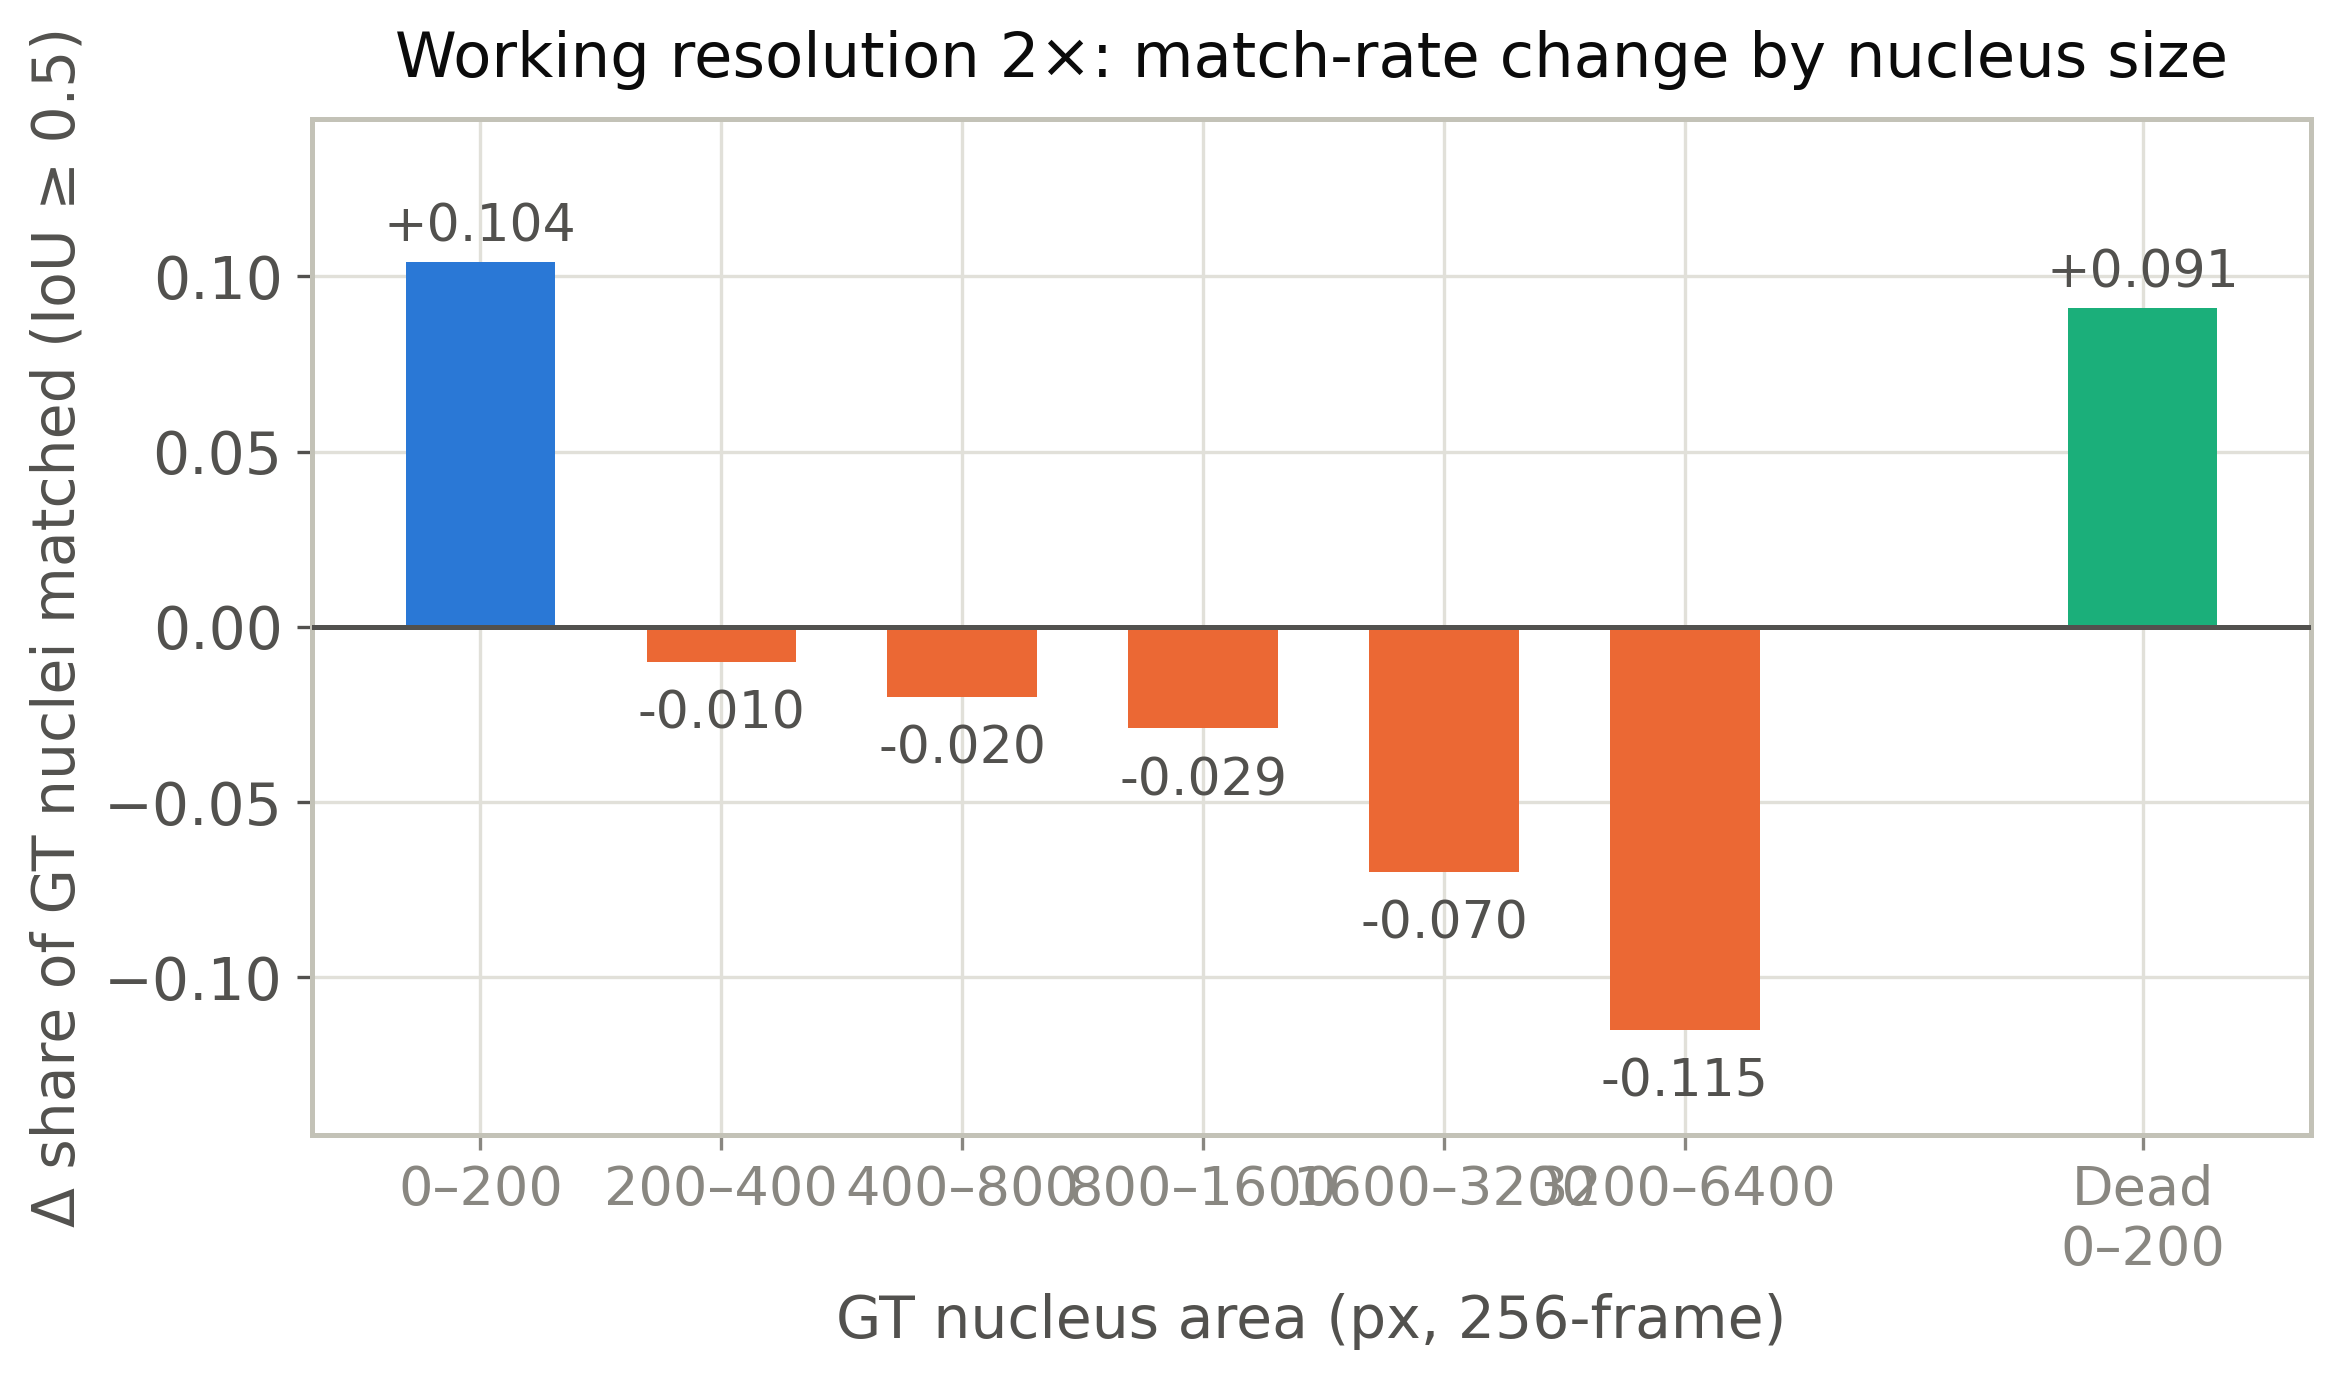
\includegraphics[width=0.88\linewidth]{figs/chart_size_bins.png}
\caption{Match-rate change from $2\times$ resolution by GT nucleus area (split-1 TTA, x2
seed 19 minus 3-seed baseline mean; IoU $\geq$ 0.5). The effect is a monotone function of
\emph{size}, not class: every nucleus below 200\,px gains (Dead included, $+$.091), every
size band above 400\,px loses, monotonically. Matched-pair IoU is flat ($\pm$.01) in every
bin.}
\label{fig:sizebins}
\end{figure}

\begin{figure}[t]
\centering
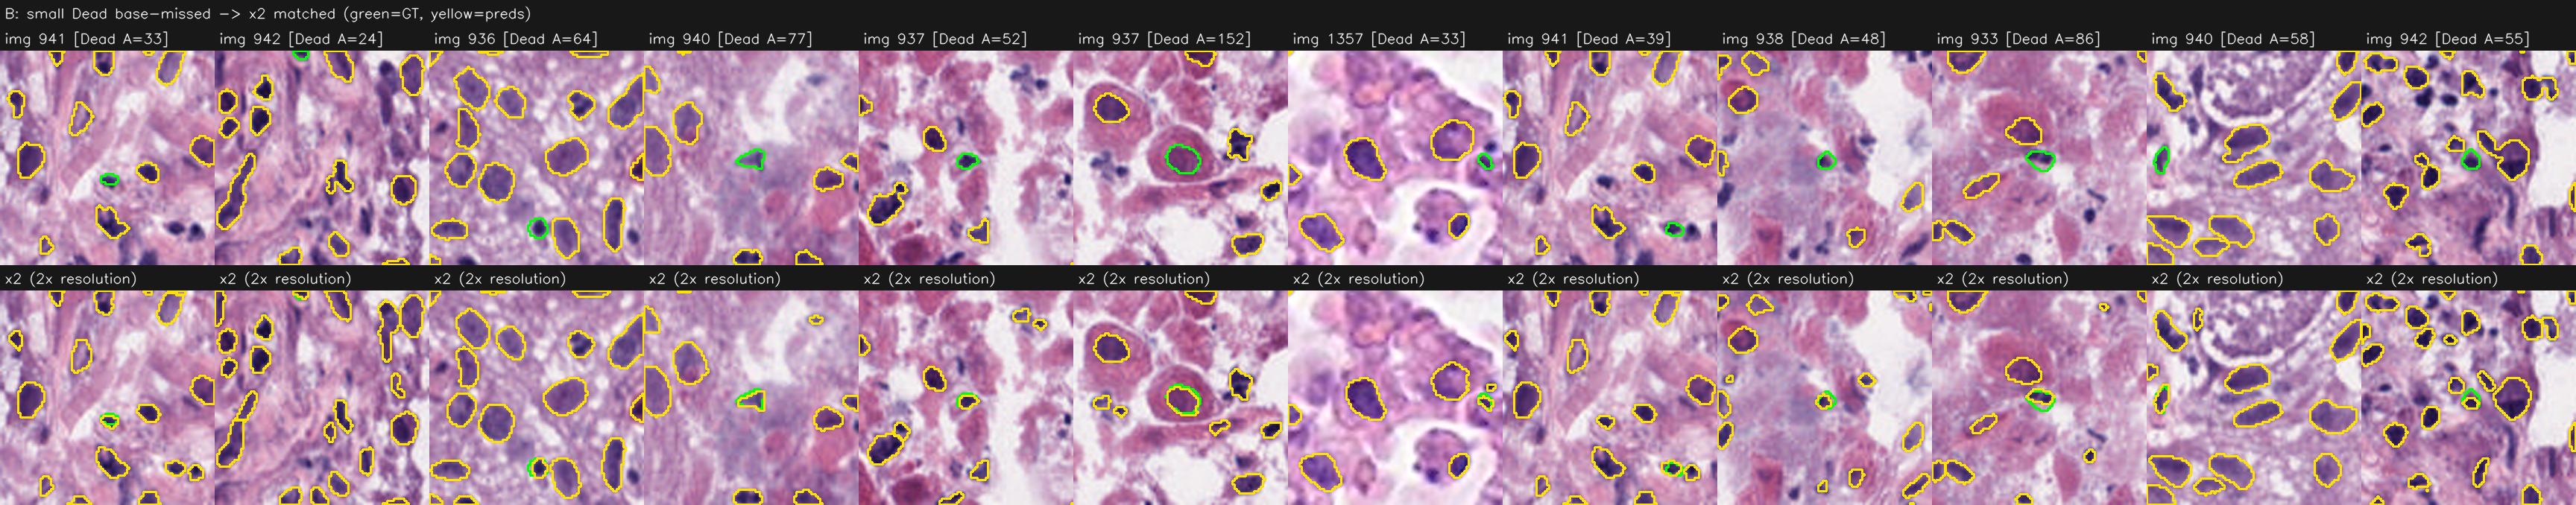
\includegraphics[width=\linewidth]{figs/x2_montage_gain.png}\\[2pt]
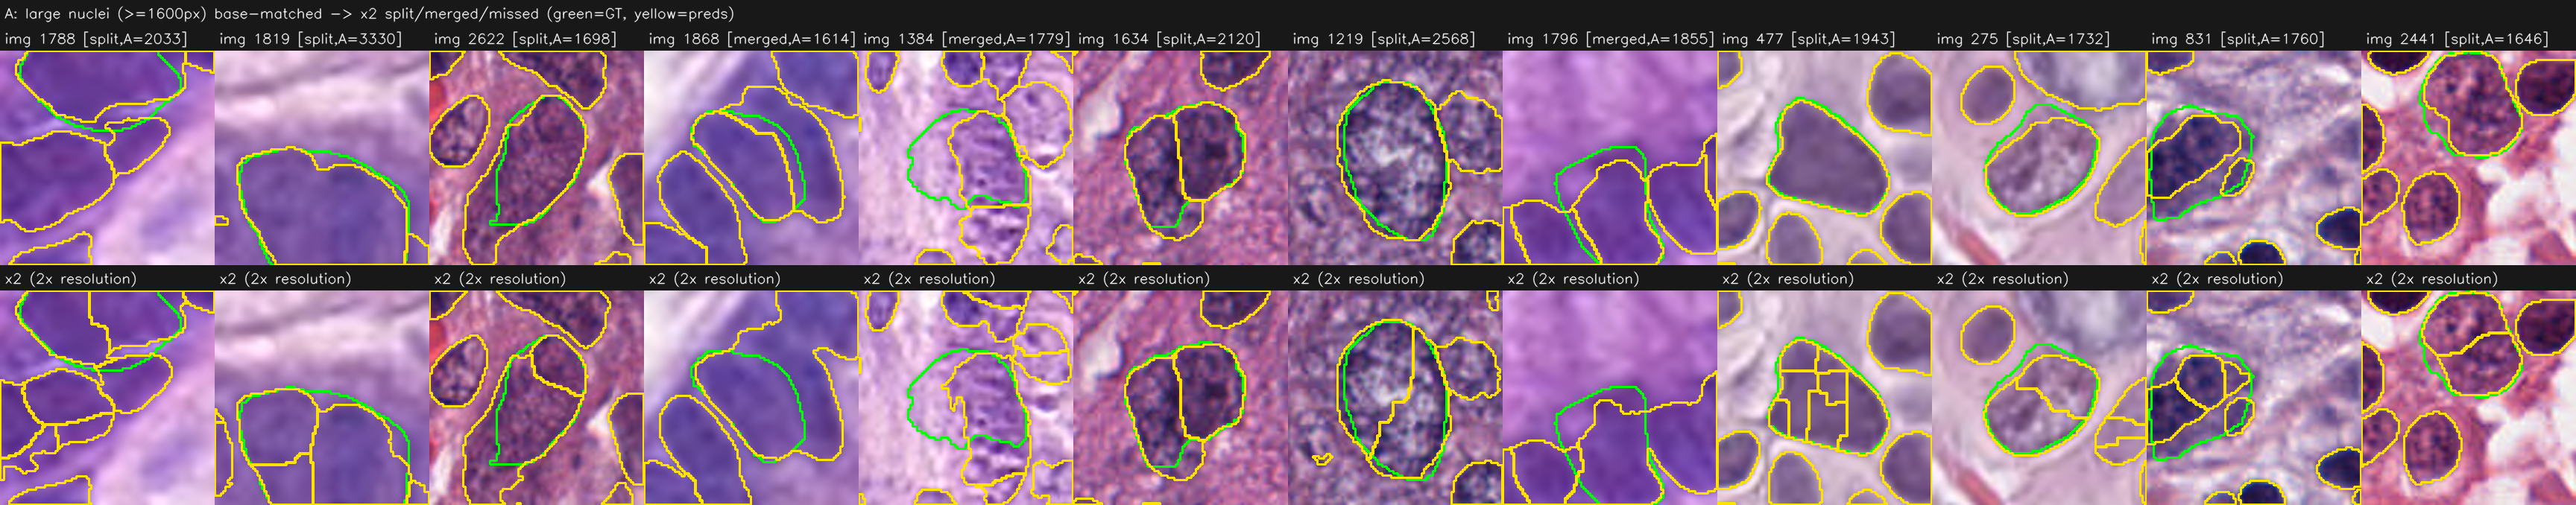
\includegraphics[width=\linewidth]{figs/x2_montage_damage.png}
\caption{Top (gains): Dead/small nuclei missed at 256 (top row of each pair: no prediction
outline) are detected at 512 (bottom row); green = ground truth, yellow = predicted
instances. Bottom (damage): large nuclei matched at 256 (single outline) fragment at 512
into interior mosaics---multiple yellow rings inside one green ring---while the outer
boundary still tracks the ground truth.}
\label{fig:montage}
\end{figure}

Three observations locate the mechanism (Figs.~\ref{fig:sizebins}--\ref{fig:montage}):

\begin{enumerate}
\item \textbf{The tax is not colocated with the Dead gain.} Across the 97 Dead-bearing test
images, corr($\Delta$Dead, $\Delta$bPQ) $=+$.23; images that gained Dead are bPQ-neutral
(median $\Delta$bPQ $+$.003), images without Dead gains carry the loss (median $-$.027). This
already rules out "Dead improvements cannibalise other classes".
\item \textbf{Size, not class, is the axis.} Match rate moves $+$.104 for non-Dead nuclei
under 200\,px (Dead 0--200: $+$.091) and declines monotonically with size to $-$.115 at
3200--6400\,px. Boundary quality of \emph{matched} nuclei is unchanged (matched-pair IoU
$\pm$.01 in every bin; missed-poor-shape rates do not grow), so nuclei are not being
matched worse---large ones are being \emph{cut into pieces}. Error composition confirms it:
GT split-rate roughly doubles in every class (Neoplastic .009$\to$.017, Connective
.013$\to$.025, Dead .010$\to$.026); among large ($\geq$1600\,px) non-Dead nuclei split goes
.072$\to$.104, merged .003$\to$.009, missed-bg .024$\to$.054; predicted-instance count rises
25.5$\to$28.4 per
image and the under-80\,px share of predictions triples (.034$\to$.109); prediction-side
fp-split roughly doubles (.019$\to$.037 pooled). Visual review of montages: 11/12 sampled
damaged large nuclei are interior-fragmentation mosaics (one nucleus $\to$ up to 7 pieces)
with the outer contour still on the ground truth, while 12/12 sampled small-Dead gains are
genuine detections (mean IoU 0.70).
\item \textbf{The obvious explanation is wrong.} "The 512$\to$256 nearest-downsample of the
instance map destroys boundaries" is refuted by the matched-IoU parity in every size bin.
The actual cause sits in the decode: HoVer-Net's post-processing applies \emph{fixed
pixel-unit constants} to the predicted maps---\texttt{remove\_small\_objects(min\_size=10)}
(area units; 2.5 native px$^2$ at $2\times$) on the blob and marker maps, and a Sobel
operator with aperture $k=21$ (10.5 native px) on the HV maps. At $2\times$ every one of
these thresholds silently \emph{relaxes} in native units: spurious markers survive on
chromatin texture and fragment large nuclei, and tiny blobs pass the size floor into the
prediction set. The small-nucleus detection gain, by contrast, is a genuine model-resolution
benefit.
\end{enumerate}

\subsection{The pre-registered decode fix ($du2$)}
\label{sec:du2}

The fix follows from the diagnosis and was registered before it was run: scale the
pixel-unit constants by the resolution factor $u$---$\mathrm{min\_size} \to 10u^2$, Sobel aperture
$\to$ the nearest odd multiple of $21u$ (41). (OpenCV caps Sobel apertures at 31; beyond
that we linearly resample the official 21-tap operator's impulse-response kernels, exact at
$u{=}1$, unit-tested bit-exact.) Re-decoding the existing checkpoints---no retraining:

\begin{table}[t]
\centering\small
\caption{$du2$ recovery (3-split means, seed 19, last checkpoint). \% = share of the
x2-vs-base gap recovered by the decode fix alone. Dead keeps its gain (and slightly grows).}
\label{tab:du2}
\begin{tabular}{llcccc}
\toprule
 & Arm & mPQ & bPQ & mPQ$^+$ & Dead PQ \\
\midrule
\multirow{3}{*}{no TTA}
 & base 256      & .4995 & .6653 & .5178 & .1760 \\
 & x2            & .4791 & .6413 & .5012 & .1816 \\
 & x2 $+$ du2    & .4894 & .6583 & .5157 & .1831 \\
\cmidrule{2-6}
 & recovered     & 50\% & 71\% & 87\% & (gain grows) \\
\midrule
\multirow{3}{*}{TTA}
 & base 256      & .5047 & .6706 & .5227 & .1767 \\
 & x2            & .4848 & .6488 & .5070 & .1786 \\
 & x2 $+$ du2    & .4926 & .6620 & .5189 & .1810 \\
\cmidrule{2-6}
 & recovered     & 39\% & 61\% & 76\% & (gain grows) \\
\bottomrule
\end{tabular}
\end{table}

\begin{figure}[t]
\centering
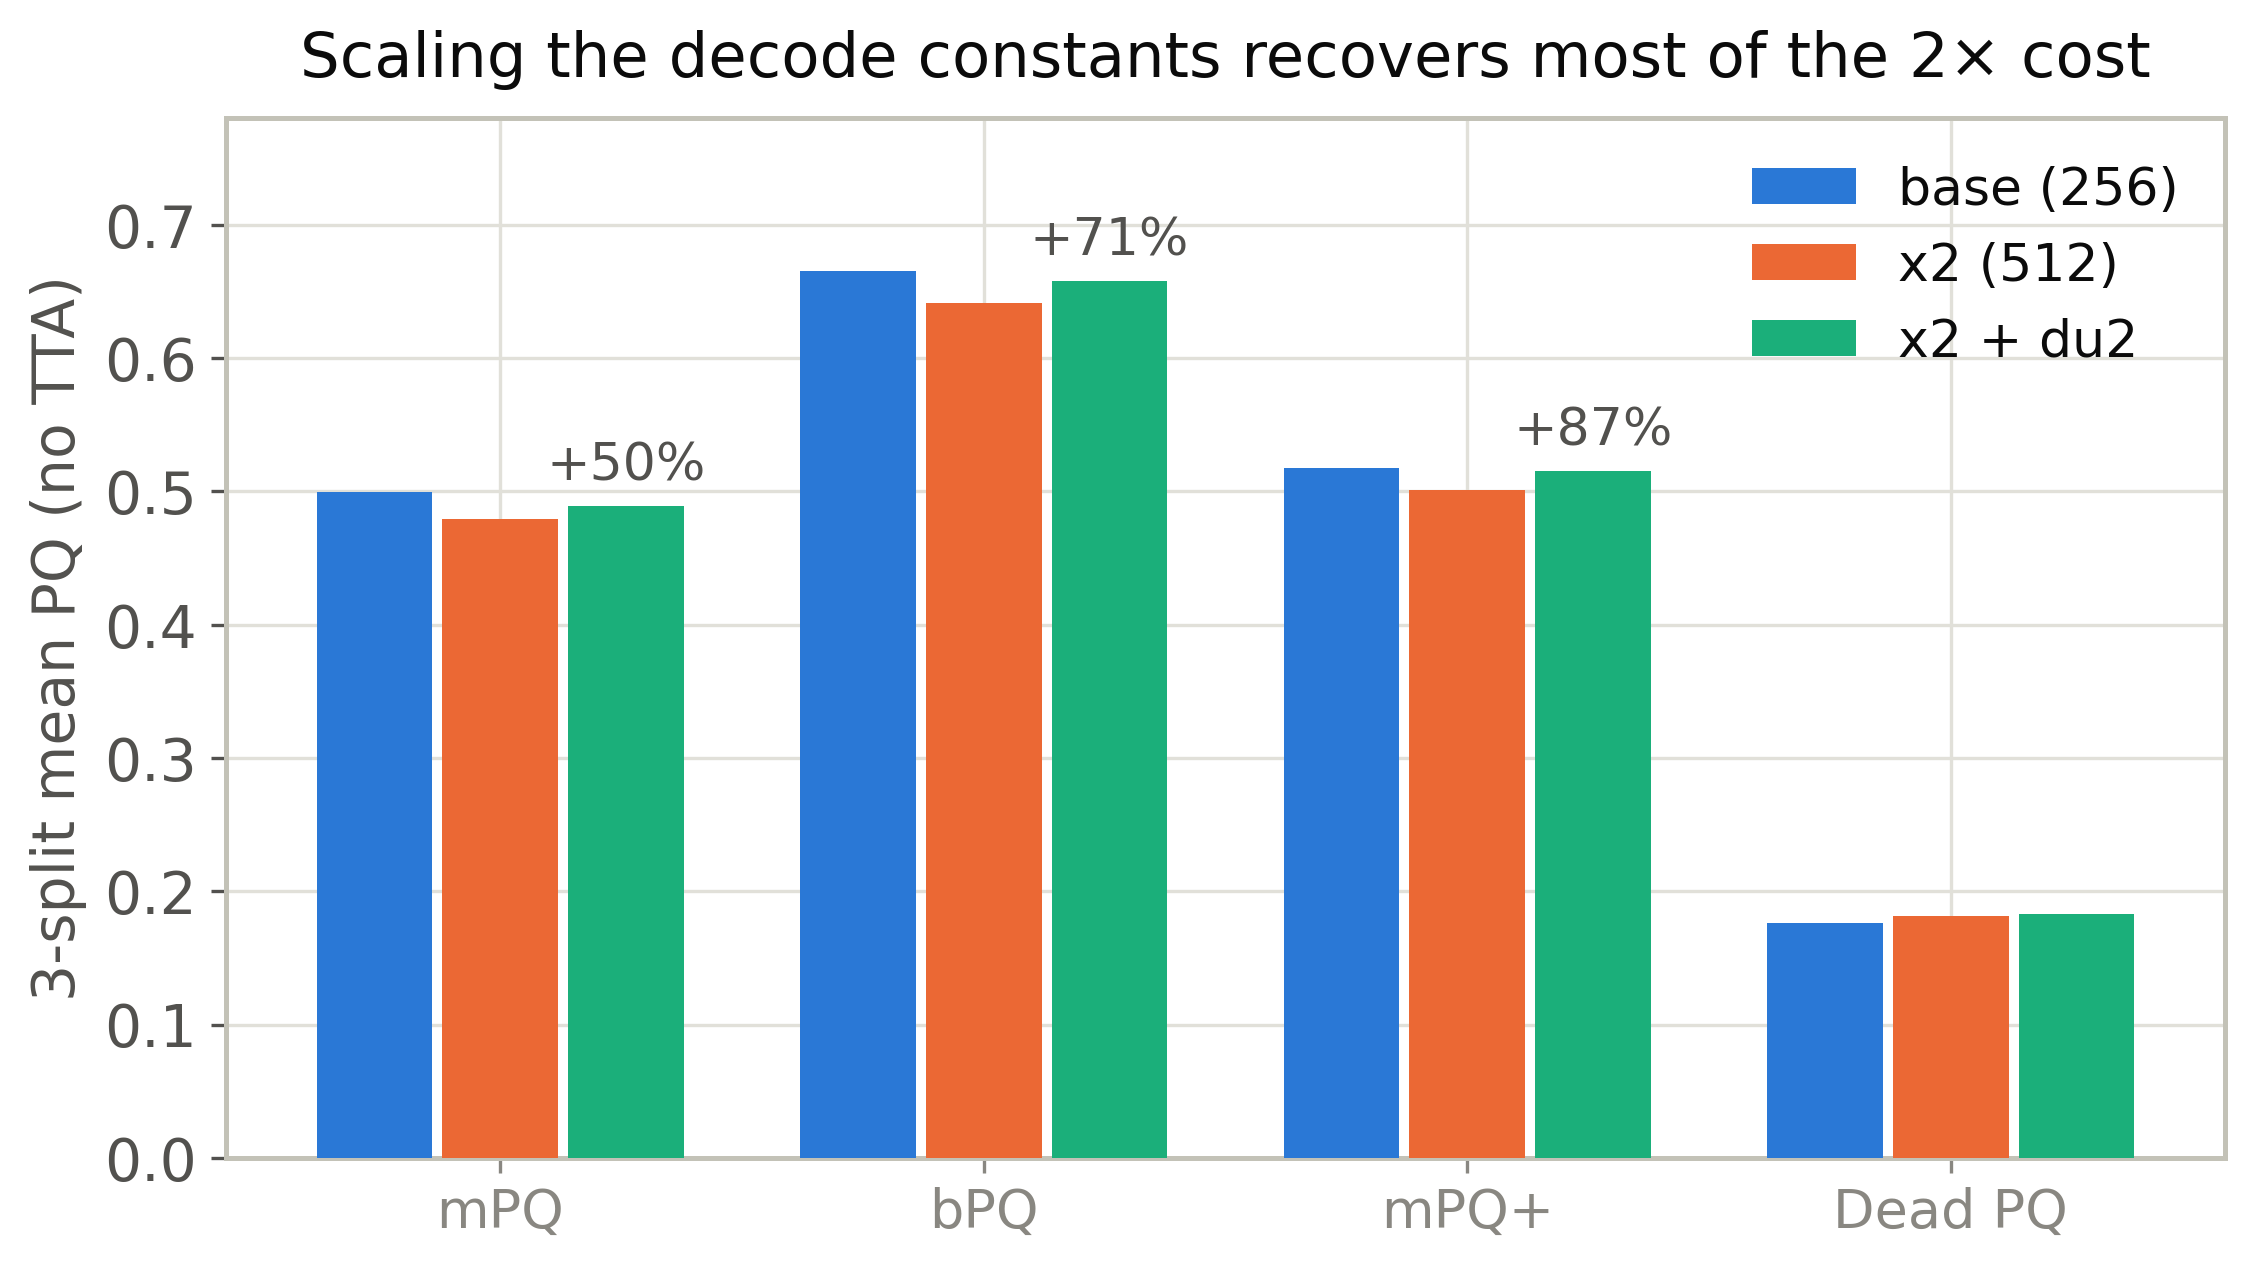
\includegraphics[width=0.86\linewidth]{figs/chart_du2_recovery.png}
\caption{Table~\ref{tab:du2} (no TTA): scaling two decode constants recovers most of the
aggregate $2\times$ cost while the Dead gain survives. mPQ$^+$ closes to within .002 of the
baseline.}
\label{fig:du2}
\end{figure}

Table~\ref{tab:du2}/Fig.~\ref{fig:du2}: the two constants account for most of the
tax---50--87\% of the mPQ/bPQ/mPQ$^+$ cost depending on metric and TTA---and the Dead gain is
kept and slightly enlarged (no-TTA $+$.006$\to+$.007), exactly as the mechanism predicted
(boundary quality
was already at parity; the Dead gain lives in detection, not decode). Per split, the x2 Dead
gain is fold-3-driven (split-1 $+$.017, split-2 $+$.009, no TTA) while split-3 (test fold 1)
shows a small loss ($-$.009) that $du2$ largely recovers ($-$.003)---consistent with the
known fold-composition asymmetry of Dead. The residual gap ($-$.007 bPQ no TTA) is genuine
fp-split at 512, not decode: scaling the third constant (the marker-open kernel, $du2mk2$)
was evaluated on validation and \emph{rejected} (worse mPQ at equal bPQ).

\subsection{A validation-only lever: strict improvement on all nine runs}
\label{sec:lever}

The visual analysis of the residual suggested two decode-side moves: merge same-class
adjacent instances (the mosaics have clean outer boundaries) and drop edge-touching slivers
(a third of the tiny FPs are border-clipping fragments). Both have free parameters, and both
were selected on \emph{validation} folds only, on the $du2$ arm, under the rule "bPQ
$\geq$ baseline $-$ .002, then max mPQ". All three splits' validation sweeps---and a fourth,
extended sweep on a decode variant---independently choose the same pair: merge fraction 0.25,
sliver area floor 40\,px.

Frozen, applied to test:

\begin{table}[t]
\centering\small
\caption{Lever verdict ($du2lev - du2$, paired image-bootstrap 95\% CIs). Top: the three
original splits (seed 19). Replication: positive mPQ and bPQ deltas on \textbf{9/9} grid runs
(Sec.~\ref{sec:grid}); Dead unchanged everywhere (CIs straddle 0).}
\label{tab:lever}
\begin{tabular}{lccc}
\toprule
Split & $\Delta$mPQ [CI] & $\Delta$bPQ [CI] & $\Delta$Dead PQ [CI] \\
\midrule
1 & $+$.0020 [$+$.0014, $+$.0026] & $+$.0030 [$+$.0022, $+$.0041] & $+$.0015 [$-$.0008, $+$.0051] \\
2 & $+$.0016 [$+$.0009, $+$.0022] & $+$.0025 [$+$.0018, $+$.0032] & $+$.0005 [$-$.0012, $+$.0028] \\
3 & $+$.0014 [$+$.0008, $+$.0021] & $+$.0021 [$+$.0014, $+$.0029] & $-$.0018 [$-$.0055, $+$.0016] \\
\bottomrule
\end{tabular}
\end{table}

Table~\ref{tab:lever}: a strict test improvement---all six mPQ/bPQ CIs exclude zero on the
positive side, every Dead view within $\pm$.002, predicted instances drop 27.2$\to$26.6 per
image (the lever removes $\sim$0.5 fragments and slivers per image and nothing else
measurable). The selection generalized with zero test-fold tuning.

\subsection{The $3{\times}3$ seed grid and the pre-registered seed-noise verdict}
\label{sec:grid}

\begin{figure}[t]
\centering
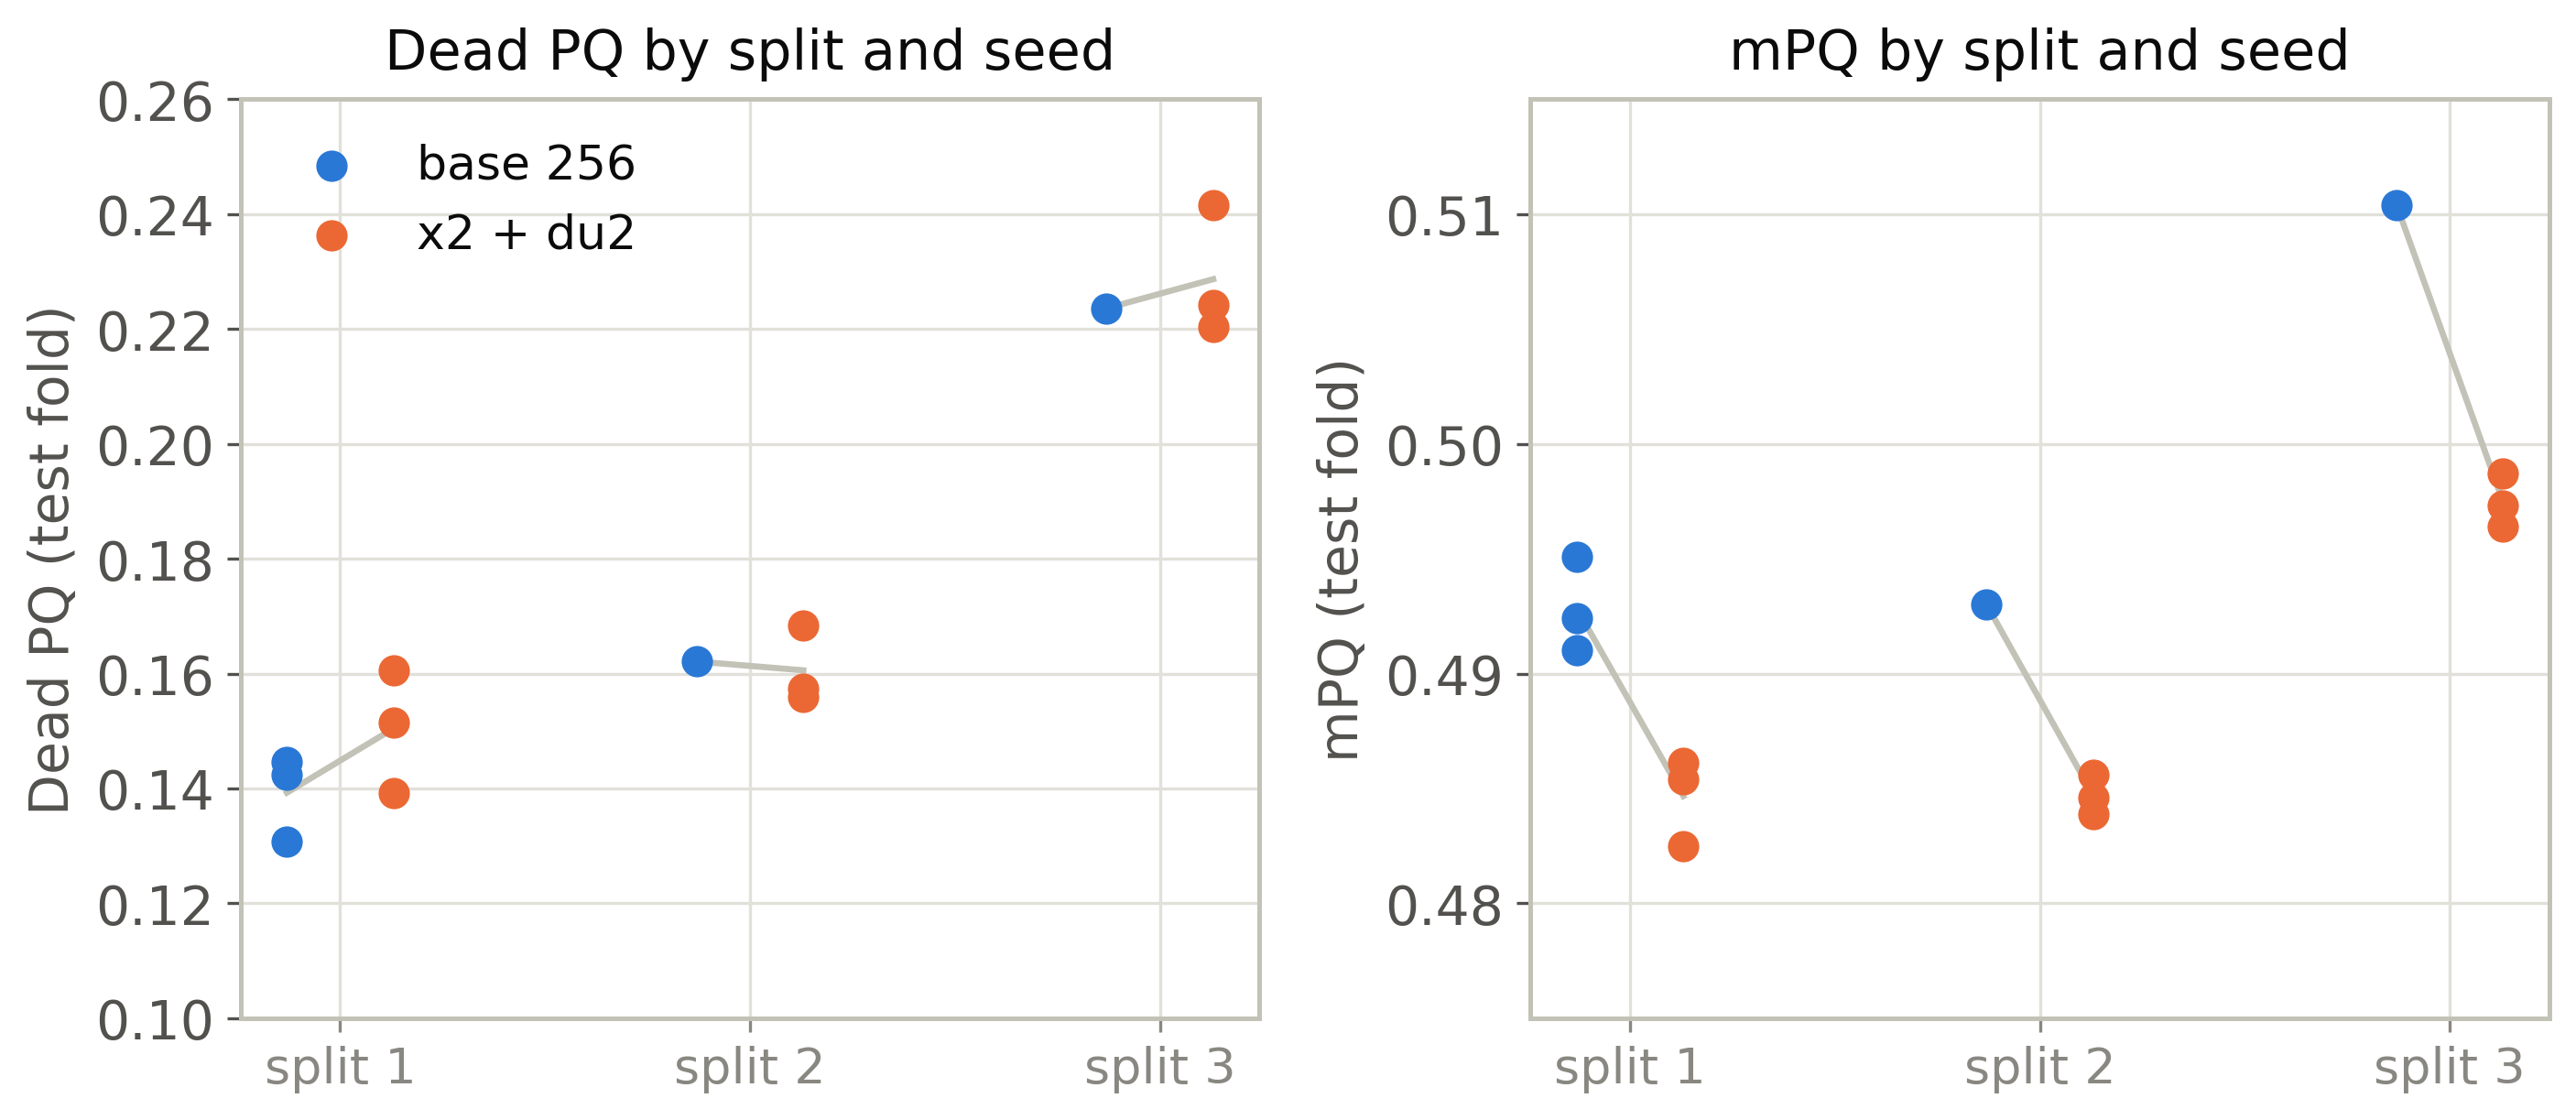
\includegraphics[width=0.98\linewidth]{figs/chart_seed_grid.png}
\caption{The seed grid. Right: mPQ---every $du2$ run (orange) sits below every baseline run
(blue) on its split; the price is unambiguous. Left: Dead PQ---runs interleave; split-2's
$du2$ seed-mean lands \emph{below} the baseline seed, split-3's seed 19 flips sign. Lines
connect seed means (baseline extra seeds exist on split 1 only).}
\label{fig:grid}
\end{figure}

\begin{table}[t]
\centering\small
\caption{$3{\times}3$ seed grid, per-split seed means $\pm$ std ($du2$ arm; baseline seeds
1/2 exist on split 1 only). Bottom: 3-split means of seed means, and the $du2lev$ arm.}
\label{tab:grid}
\begin{tabular}{llccc}
\toprule
Split & Arm & mPQ & bPQ & Dead PQ \\
\midrule
\multirow{2}{*}{1} & base   & .4928 $\pm$ .0021 & .6661 $\pm$ .0015 & .1393 $\pm$ .0074 \\
                   & du2    & .4846 $\pm$ .0019 & .6565 $\pm$ .0003 & .1504 $\pm$ .0107 \\
\midrule
\multirow{2}{*}{2} & base   & .4930 & .6638 & .1621 \\
                   & du2    & .4847 $\pm$ .0009 & .6568 $\pm$ .0005 & .1606 $\pm$ .0068 \\
\midrule
\multirow{2}{*}{3} & base   & .5104 & .6647 & .2236 \\
                   & du2    & .4975 $\pm$ .0012 & .6605 $\pm$ .0013 & .2287 $\pm$ .0112 \\
\midrule
\multirow{3}{*}{3-split} & base   & .4987 & .6648 & .1750 \\
                         & du2    & .4889 & .6579 & .1799 \\
                         & du2lev & .4905 & .6603 & .1801 \\
\bottomrule
\end{tabular}
\end{table}

The grid (Table~\ref{tab:grid}, Fig.~\ref{fig:grid}) exists for one purpose: the
pre-registered seed-noise verdict, which compares each Line-B effect against the per-seed
standard deviation of the identical recipe.

\begin{itemize}
\item \textbf{The prices are seed-robust.} $\Delta$mPQ $-$0.0098 and $\Delta$bPQ $-$0.0069
($du2$ vs base, 3-split means) are $4.7\times$ and $5.3\times$ the largest per-split seed
std (0.0021 / 0.0013), same sign on every one of the 9 runs. x1 stays ahead on mPQ/bPQ at
$\sim$5$\times$ seed noise.
\item \textbf{The Dead gain is fragile.} $+$.0049 on 3-split means is only
$0.4$--$0.7\times$ the per-seed Dead std (0.0068--0.0112). Paired same-seed comparisons
favor $du2$ on 4 of 5 pairs (split-3 seed 19 flips, $-$.0032), and split-level seed means go
$+$.0111 (split 1, 3/3 seeds) / $-$.0015 (split 2, flips) / $+$.0051 (split 3, 2/3). The x2
Dead advantage is real on split 1, present-but-noisy on split 3, a wash on split 2.
\end{itemize}

\subsection{Final standing: the priced trade}
\label{sec:final}

Table~\ref{tab:arch}, bottom block, collects the final standing (3-split means, seed 19, no
TTA): the levered $2\times$ arm trades $-$.0085 mPQ / $-$.0045 bPQ for interior-Dead miss
$-$.070 ($0.372\!\to\!0.302$), Dead $F_c$ $+$.034, Dead DQ$^+$ $+$.026, Uterus-excluded Dead
PQ $+$.009, and interior-Dead matched share $+$.07; mPQ$^+$ is at parity ($-$.0005 on the
pooled grid; $-$.0007 seed 19). Per the pre-registered combined endpoint, $2\times$ working
resolution with the corrected decode is \textbf{not a default win}---it is an explicitly
priced trade, and the price is now fully accounted for: decode constants ($du2$)
$\approx$two-thirds of the bPQ tax, the lever another eighth, the residual $\approx$genuine
fp-split at 512.

\section{Discussion}
\label{sec:discussion}

\paragraph{Why detection-first does not fix Dead.} Line A's two results have one shape.
KongNet's detector finds Dead nuclei (per-nucleus $F_c$ mid-pack) but its decode fuses
touching same-class nuclei, and Dead's failure geometry \emph{is} touching same-class
clusters; LKCell-L separates and matches instances better (bPQ, mPQ$^+$, Dead $F_c$ all up)
but its detected Dead nuclei fail type pairing, so detection gains do not become Dead PQ.
Together with report I's negative results, the picture is now: the Dead deficit is not a
property of one decoder family, and it is not closed by any published architecture under a
matched protocol. What \emph{moves} it is resolution---which brings more pixels to bear on
small nuclei---and even that helps detection while leaving the separation and typing of what
is detected to the same machinery as before.

\paragraph{Pixel-unit constants are a first-class confound.} The $du2$ result has an
implication beyond this project: every pipeline built on HoVer-Net's post-processing (which
is most of the field) carries resolution-hardcoded constants. Any resolution, patch-size, or
backbone-stride change silently re-scales the effective decode; published resolution
ablations that do not correct for it measure the change \emph{plus} an artifact biased
against higher resolution. We found no discussion of this in the nuclei-segmentation
literature; the two-line fix is in our repository's decode.

\paragraph{Honest effect sizes, pre-registered.} The seed grid separates what survives
pooling from what does not. The prices survive at $\sim$5$\times$ seed noise with uniform
sign; the Dead PQ gain does not survive at all as a headline ($0.4$--$0.7\times$ seed std,
one split flipped). What \emph{is} solid on the Dead side are the detection-geometry
endpoints---interior-Dead miss $-$.070 and Dead $F_c$ $+$.034, replicated in sign on every
run---while the class-PQ aggregation over 65--97 Dead-bearing images remains the noisiest
measurement in the benchmark. This is report I's noise calibration doing its job: the
headline number is not the one to trust, and we say which one is.

\paragraph{Evaluation recipes, again.} LKCell-L is the second released model (after
HoVer-NeXt-T in report I) whose published numbers exceed our strict re-evaluation by more
than typical leaderboard gaps ($\sim$0.015 uniform), and KongNet's headline Dead advantage
does not survive validation-tuned decoding at all. Both gaps are protocol, not pipeline:
everything reproduces cleanly once the recipe is matched. The leaderboard's meaningful
resolution is finer than its recipes.

\section{Status and Remaining Work}
\label{sec:status}

Line A and Line B are complete and closed (A negative; B a priced, fully-replicated trade
with the mechanism accounted for). Remaining before the final report: strict re-evaluation of
the remaining released per-fold weights (PromptNucSeg, CellVTA), extending the cross-domain
rank pool from four architectures to six; the final report's figure set (tissue$\times$class
heatmaps, error decomposition across architectures); optional additional external sets
(MoNuSeg, NuInsSeg); and the phase-2 data direction (larger leak-free training data, pooled
external Dead labels) which remains unstarted and is the main open lever for Dead beyond
resolution.

\begin{thebibliography}{99}\small
\bibitem{gamper2019pannuke} J.~Gamper, N.~Alemi~Koohbanani, K.~Benet, A.~Khuram, N.~Rajpoot,
``PanNuke: An Open Pan-Cancer Histology Dataset for Nuclei Instance Segmentation and
Classification,'' \emph{ECDP}, LNCS 11435, pp.~11--19, 2019; and J.~Gamper et al., ``PanNuke
Dataset Extension, Insights and Baselines,'' arXiv:2003.10778, 2020.
\bibitem{graham2019hovernet} S.~Graham, Q.~D.~Vu, S.~E.~Raza, A.~Azam, Y.-W.~Tsang,
J.~Kwak, N.~Rajpoot, ``HoVer-Net: Simultaneous Segmentation and Classification of Nuclei in
Multi-Tissue Histology Images,'' \emph{Medical Image Analysis}, 58:101563, 2019.
\bibitem{horta2024cellvit} F.~H\"orst, M.~Rempe, L.~Heine, J.~Kleesiek, ``CellViT: Vision
Transformers for Precise Cell Segmentation and Classification,'' \emph{Medical Image
Analysis}, 94:103143, 2024.
\bibitem{horta2025cellvitpp} F.~H\"orst, M.~Rempe, H.~Becker, L.~Heine, J.~Keyl, J.~Kleesiek,
``CellViT++: Energy-Efficient and Adaptive Cell Segmentation and Classification Using
Foundation Models,'' \emph{Computer Methods and Programs in Biomedicine}, 277:109206, 2026.
\bibitem{hovenext} E.~Baumann, B.~Dislich, J.~L.~Rumberger, J.~L.~Nagtegaal,
M.~Rodr\'iguez~Mart\'inez, I.~Zlobec, ``HoVer-NeXt: A Fast Nuclei Segmentation and
Classification Pipeline for Next Generation Histopathology,'' \emph{MIDL}, PMLR 250:61--86,
2024.
\bibitem{promptnucseg} Z.~Shui, Y.~Zhang, K.~Yao, C.~Zhu, S.~Zheng, J.~Li, H.~Li, Y.~Sun,
R.~Guo, L.~Yang, ``Unleashing the Power of Prompt-Driven Nucleus Instance Segmentation
(PromptNucSeg),'' \emph{ECCV}, LNCS 15085, pp.~288--304, 2024.
\bibitem{lv2025kongnet} J.~Lv, E.~S.~Nasir, K.~Xu, M.~Jahanifar, B.~S.~Chohan,
B.~Elhaminia, S.~E.~A.~Raza, ``KongNet: A Multi-headed Deep Learning Model for Detection and
Classification of Nuclei in Histopathology Images,'' arXiv:2510.23559, 2025.
\bibitem{cui2024lkcell} Z.~Cui, J.~Yao, L.~Zeng, J.~Yang, W.~Liu, X.~Wang, ``LKCell:
Efficient Cell Nuclei Instance Segmentation with Large Convolution Kernels,''
arXiv:2407.18054, 2024.
\end{thebibliography}

\end{document}
